\documentclass[oneside,10pt]{book}
\usepackage{graphicx} % Required for inserting images
\usepackage[T1]{fontenc} % Nice font rendering
\usepackage[a4paper, portrait, margin=1.5in]{geometry}

% Math
\usepackage{amsmath,amssymb,amsthm,derivative}
\usepackage{txfonts,times}
\usepackage{mathtools}
\usepackage{xparse}

%   Expectation
    \NewDocumentCommand{\expect}{ O{} e{_} s o >{\SplitArgument{1}{|}}m }{%
      \operatorname{\mathbb{E}}%     the variance operator
      \IfValueT{#2}{_{{#2}}}% subscript immediately after Var
      \IfValueT{#1}{^{\mathbb{#1}}}% superscript immediately after Var
      \IfBooleanTF{#3}{% *-variant
        \expectarg*{\expectvar#5}%
      }{% no *-variant
        \IfNoValueTF{#4}{% no optional argument
          \expectarg{\expectvar#5}%
        }{% optional argument
          \expectarg[#4]{\expectvar#5}%
        }%
      }%
    }
    \NewDocumentCommand{\expectvar}{mm}{%
      #1\IfValueT{#2}{\nonscript\;\delimsize\vert\nonscript\;#2}%
    }
    \DeclarePairedDelimiterX{\expectarg}[1]{[}{]}{#1}



%   Variance
    \NewDocumentCommand{\var}{ O{} e{_} s o >{\SplitArgument{1}{|}}m }{%
      \operatorname{\mathrm{var}}%     the variance operator
      \IfValueT{#2}{_{{#2}}}% subscript immediately after Var
      \IfValueT{#1}{^{\mathbb{#1}}}% superscript immediately after Var
      \IfBooleanTF{#3}{% *-variant
        \vararg*{\varvar#5}%
      }{% no *-variant
        \IfNoValueTF{#4}{% no optional argument
          \vararg{\varvar#5}%
        }{% optional argument
          \vararg[#4]{\varvar#5}%
        }%
      }%
    }
    \NewDocumentCommand{\varvar}{mm}{%
      #1\IfValueT{#2}{\nonscript\;\delimsize\vert\nonscript\;#2}%
    }
    \DeclarePairedDelimiterX{\vararg}[1]{(}{)}{#1}


%   Covariance
    \NewDocumentCommand{\cov}{ O{} e{_} s o >{\SplitArgument{1}{|}}m }{%
      \operatorname{\mathrm{cov}}%     the covariance operator
      \IfValueT{#2}{_{{#2}}}% subscript immediately after Cov
      \IfValueT{#1}{^{\mathbb{#1}}}% superscript immediately after Cov
      \IfBooleanTF{#3}{% *-variant
        \covarg*{\covvar#5}%
      }{% no *-variant
        \IfNoValueTF{#4}{% no optional argument
          \covarg{\covvar#5}%
        }{% optional argument
          \covarg[#4]{\covvar#5}%
        }%
      }%
    }
    \NewDocumentCommand{\covvar}{mm}{%
      #1\IfValueT{#2}{\nonscript\;\delimsize\vert\nonscript\;#2}%
    }
    \DeclarePairedDelimiterX{\covarg}[1]{(}{)}{#1}


%   Correlation
    \NewDocumentCommand{\corr}{ O{} e{_} s o >{\SplitArgument{1}{|}}m }{%
      \operatorname{\mathrm{corr}}%     the correlation operator
      \IfValueT{#2}{_{{#2}}}% subscript immediately after Corr
      \IfValueT{#1}{^{\mathbb{#1}}}% superscript immediately after Corr
      \IfBooleanTF{#3}{% *-variant
        \corrarg*{\corrvar#5}%
      }{% no *-variant
        \IfNoValueTF{#4}{% no optional argument
          \corrarg{\corrvar#5}%
        }{% optional argument
          \corrarg[#4]{\corrvar#5}%
        }%
      }%
    }
    \NewDocumentCommand{\corrvar}{mm}{%
      #1\IfValueT{#2}{\nonscript\;\delimsize\vert\nonscript\;#2}%
    }
    \DeclarePairedDelimiterX{\corrarg}[1]{(}{)}{#1}


%   Probability with measure
    \NewDocumentCommand{\prob}{ O{} e{_} s o >{\SplitArgument{1}{|}}m }{%
      \operatorname{\mathbb{#1}}%     the correlation operator
      \IfValueT{#2}{_{{#2}}}% subscript immediately after prob
      \IfBooleanTF{#3}{% *-variant
        \probarg*{\probvar#5}%
      }{% no *-variant
        \IfNoValueTF{#4}{% no optional argument
          \probarg{\probvar#5}%
        }{% optional argument
          \probarg[#4]{\probvar#5}%
        }%
      }%
    }
    \NewDocumentCommand{\probvar}{mm}{%
      #1\IfValueT{#2}{\nonscript\;\delimsize\vert\nonscript\;#2}%
    }
    \DeclarePairedDelimiterX{\probarg}[1]{(}{)}{#1}


%   Quadratic Variation
    % Quadratic Variation with Auto-adjusting Brackets
    \NewDocumentCommand{\quadvar}{ m }{%
      \left\langle #1 \right\rangle%
    }
%   Norm
    \DeclarePairedDelimiter{\norm}{\lVert}{\rVert}

%   Absolute value
    \DeclarePairedDelimiter{\abs}{\lvert}{\rvert}

%   Inner product
    \DeclarePairedDelimiterX{\inner}[2]{\langle}{\rangle}{#1, #2}

%   Argmax
    \NewDocumentCommand{\argmax}{ e{_} }{%
      \operatorname*{argmax}%     the argmax operator
      \IfValueT{#1}{_{#1}}% subscript immediately after argmax
    }

%   Argmin
    \NewDocumentCommand{\argmin}{ e{_} }{%
      \operatorname*{argmin}%     the argmax operator
      \IfValueT{#1}{_{#1}}% subscript immediately after argmax
    }

%   Indicator
    \NewDocumentCommand{\ind}{ e{_} }{%
      \operatorname{\mathbf 1}%     the argmax operator
      \IfValueT{#1}{_{\{#1\}}}% subscript immediately after argmax
    }
\newtheorem{theorem}{Theorem}[chapter]
\newtheorem{lemma}[theorem]{Lemma}
\newtheorem{corollary}[theorem]{Corollary}

\theoremstyle{definition}
\newtheorem{definition}[theorem]{Definition}

\theoremstyle{definition}
\newtheorem{example}{Example}[chapter]

\theoremstyle{remark}
\newtheorem*{remark}{Remark}

\theoremstyle{definition}
\newtheorem{exercise}{Exercise}[chapter]

\theoremstyle{definition}
\newtheorem{solution}{Solution}[chapter]


\usepackage{varioref}
\usepackage{hyperref}
\usepackage{cleveref}   % in this order please
\usepackage{tikz} % Diagrams
\usepackage{enumerate} % numbered bullet points
\usepackage[shortlabels]{enumitem}
\usepackage{xcolor}

% CODE
\usepackage{listings}
\usepackage[most]{tcolorbox}
\usepackage{inconsolata}

\newtcblisting[auto counter]{sexylisting}[2][]{sharp corners, 
    fonttitle=\bfseries, colframe=gray, listing only, 
    listing options={basicstyle=\ttfamily,language=java}, 
    title=Listing \thetcbcounter: #2, #1}


\title{EC2C3 Econometrics I}
\date{July 2024}
\author{Nimar C. Zhao\footnote{Department of Economics, London School of Economics and Political Science}}

\begin{document}
\maketitle
\tableofcontents
\newpage

\chapter{Selection}
    \section{Potential Outcomes Framework}
        \subsection{Potential outcome}
            When thinking about the possible effect of a treatment, we need to understand the concept of \textit{potential outcomes}. Inherently, each individual has two \textit{potential outcomes} as defined below.
            \begin{definition}[Potential outcome]
                The \textit{potential outcomes} of $Y_i$ represent the underlying outcomes that would occur if treated or not treated,
                \begin{align}
                    \text{potential outcomes of } Y_i=\begin{cases}
                        Y_{1i}  &\text{"outcome if treated"}   \\
                        Y_{0i}  &\text{"outcome if not treated"}
                    \end{cases}
                \end{align}
            \end{definition}

        \subsection{Observed outcome}
            In reality, we can only actually observe one of the potential outcomes. Let $D_i$ track whether a individual $i$ is treated or not; $D_i = 1$ denotes treated, while $D_i = 0$ means untreated. $D_i$ is an example of what we call a \textit{dummy variable}. 
            \begin{definition}[Observed outcome]
                The \textit{observed outcome} of $Y_i$, simply denoted by $Y_i$, depends on $D_i$ through
                \begin{align}
                    \text{observed outcome, } Y_i &=
                    \begin{cases}
                        Y_{1i}  &\text{if }D_i=1\\
                        Y_{0i}  &\text{if }D_i=0
                    \end{cases}
                \end{align}
                or alternatively, $Y_i = Y_{0i}+D_i\,(Y_{1i}-Y_{0i})$.
            \end{definition}

            In addition, the opposite of the observed outcome is termed the \textit{counterfactual outcome}, i.e. the outcome not observed. For example, if $D_i = 1$ we therefore observe $Y_i = Y_{1i}$, and so $Y_{0i}$ is the counterfactual outcome. The meaning in full can be expressed as
            \begin{quote}
                `The result if individual $i$ (who had actually been treated), had not received treatment'
            \end{quote}

        \subsection{Treatment effects}
            For an individual, the true effect of treatment is $Y_{1i} - Y_{0i}$; but as we discussed above, we can virtually never observe this. In addition, treatment effects may vary from individual to individual. Therefore when analysing experimental results, we would like to understand the effect of treatment on aggregate, defined as ATE below. This is not always possible, and so there are some other similar intuitive concepts defined below:
            \begin{definition}[Average treatment effects]
                We consider three types of average treatment effects.
                \begin{enumerate}
                    \item Average Treatment Effect, ATE $:= \expect{Y_{1i} - Y_{0i}}$
                    \item Average Treatment Effect on the Treated, ATT $:= \expect{Y_{1i} - Y_{0i}| D_i = 1}$
                    \item Average Treatment Effect on the Untreated, ATU $:= \expect{Y_{1i} - Y_{0i}| D_i = 0}$
                \end{enumerate}
            \end{definition}


    \section{The selection problem}
        For us econometricians, we would ideally like to infer the treatment effect for all $i$, $Y_{1i}-Y_{0i}$ or at least the expectation, $\expect{Y_{1i}-Y_{0i}}$. However for an individual, we can’t observe both $Y_{1i}$ and $Y_{0i}$ — depending on the treatment, one must be counterfactual, as discussed above. This is the basic premise of the \textit{selection problem}.

        Before we attempt to tackle this problem, we briefly summarise the quantities that we do actually have:
        \begin{itemize}
            \item $\expect{Y_{1i}|D_i = 1}$ – treatment outcome (for those treated)
            \item $\expect{Y_{0i}|D_i = 0}$ - untreated outcome (for those not treated)
        \end{itemize}
        Based on this, we define the \textit{observed difference} below.
        \begin{definition}[Observed difference]
            The \textit{observed/naïve difference} is defined as
            \begin{align}
                \text{observed difference} := \expect{Y_{1i}|D_i = 1} - \expect{Y_{0i}|D_i = 0}
            \end{align}
            It is the difference in outcomes between the treated group and the untreated group.
        \end{definition}


        \subsection{Selection bias}
            Even without treatment, those who were supposed to be treated may see a difference with the outcome of those who did not receive treatment; this is the idea behind selection bias.

            \begin{definition}[Selection bias]
                \textit{Selection bias} is the difference in untreated outcomes between treatment and untreated groups, defined by
                \begin{align}
                    \text{selection bias} := \expect{Y_{0i}|D_i = 1} - \expect{Y_{0i}|D_i = 0}
                \end{align}
                It represents the inherent baseline difference between the two groups. Note this is not directly observed as the first term is counterfactual.
            \end{definition}

            An important property of the observed difference is discussed in the following theorem:
            \begin{theorem}
                The observed difference can be decomposed into
                \begin{align}
                    \mathrm{observed}\text{ }\mathrm{difference} = \mathrm{ATT} + \mathrm{selection}\text{ }\mathrm{bias}
                \end{align}
            \end{theorem}
            \begin{proof}
                We have
                \begin{align*}
                    \text{observed difference}
                        &:= \expect{Y_{1i}|D_i=1} - \expect{Y_{0i}|D_i=0}   \\
                        &= \expect{Y_{1i}|D_i=1} \\
                        &\phantom{=}\qquad\underbrace{- \expect{Y_{0i}|D_i = 1} + \expect{Y_{0i}|D_i = 1}}_{=0} - \expect{Y_{0i}|D_i=0}    \\
                        &= \expect{Y_{1i} - Y_{0i}|D_i=1} - \left(\expect{Y_{0i}|D_i = 1} - \expect{Y_{0i}|D_i = 0}\right)  \\
                        &= \text{ATT} + \text{selection bias}
                \end{align*}
            \end{proof}

        \subsection{Confounders}
            Why may selection bias arise? One answer comes from confounders.
            \begin{definition}[Confounder]
                A \textit{confounder} is a common factor that is correlated with both the treatment and outcome. Graphically we can view this as another variable, $Z$ in Figure \ref{fig:selection/confounders}.
            \end{definition}

            \begin{figure}[h]
                \centering
                
\tikzset{every picture/.style={line width=0.75pt}} %set default line width to 0.75pt        

\begin{tikzpicture}[x=0.75pt,y=0.75pt,yscale=-1,xscale=1]
%uncomment if require: \path (0,361); %set diagram left start at 0, and has height of 361

%Rounded Rect [id:dp7232682276583055] 
\draw   (230,168) .. controls (230,163.58) and (233.58,160) .. (238,160) -- (312,160) .. controls (316.42,160) and (320,163.58) .. (320,168) -- (320,192) .. controls (320,196.42) and (316.42,200) .. (312,200) -- (238,200) .. controls (233.58,200) and (230,196.42) .. (230,192) -- cycle ;

%Rounded Rect [id:dp7900793201983274] 
\draw   (320,98) .. controls (320,93.58) and (323.58,90) .. (328,90) -- (402,90) .. controls (406.42,90) and (410,93.58) .. (410,98) -- (410,122) .. controls (410,126.42) and (406.42,130) .. (402,130) -- (328,130) .. controls (323.58,130) and (320,126.42) .. (320,122) -- cycle ;

%Rounded Rect [id:dp49000656757418604] 
\draw   (140,98) .. controls (140,93.58) and (143.58,90) .. (148,90) -- (222,90) .. controls (226.42,90) and (230,93.58) .. (230,98) -- (230,122) .. controls (230,126.42) and (226.42,130) .. (222,130) -- (148,130) .. controls (143.58,130) and (140,126.42) .. (140,122) -- cycle ;

%Straight Lines [id:da16218237230483512] 
\draw    (320,160) -- (359.5,133.66) ;
\draw [shift={(362,132)}, rotate = 146.31] [fill={rgb, 255:red, 0; green, 0; blue, 0 }  ][line width=0.08]  [draw opacity=0] (8.93,-4.29) -- (0,0) -- (8.93,4.29) -- cycle    ;
%Straight Lines [id:da880895933850384] 
\draw    (230,160) -- (189.57,135.55) ;
\draw [shift={(187,134)}, rotate = 31.16] [fill={rgb, 255:red, 0; green, 0; blue, 0 }  ][line width=0.08]  [draw opacity=0] (8.93,-4.29) -- (0,0) -- (8.93,4.29) -- cycle    ;
%Straight Lines [id:da6515543213351532] 
\draw    (235,110) -- (312,110) ;
\draw [shift={(315,110)}, rotate = 180] [fill={rgb, 255:red, 0; green, 0; blue, 0 }  ][line width=0.08]  [draw opacity=0] (8.93,-4.29) -- (0,0) -- (8.93,4.29) -- cycle    ;

% Text Node
\draw (176,101.4) node [anchor=north west][inner sep=0.75pt]    {$D_{i}$};
% Text Node
\draw (267,171.4) node [anchor=north west][inner sep=0.75pt]    {$Z_{i}$};
% Text Node
\draw (358,102.4) node [anchor=north west][inner sep=0.75pt]    {$Y_{i}$};


\end{tikzpicture}
                \caption{Confounders}
                \label{fig:selection/confounders}
            \end{figure}

            How does this relate to selection bias? For example, if the treatment $D_i$ was `health insurance' and outcome variable was `health', then a confounder could be `education'. Education may improve both an individual’s probability of taking health insurance and health outcomes, hence the observed difference is unlikely to be an accurate depiction of the effect of health insurance on health outcomes.


        \subsection{Random assignment}
            Suppose we randomly assign treatment, meaning $Y_{0i}$ and $Y_{1i}$ are independent of $D_i$. From rules of conditional expectation, this means for $j,d\in\{0,1\}$,
            \begin{align}
                \expect{Y_{ji} | D_i = d} = \expect{Y_{ji}}
            \end{align}

            \begin{theorem}
                Under random treatment assignment, the observed difference is equal to the average treatment effect (ATE); that is selection bias is zero.
            \end{theorem}
            \begin{proof}
                Consider the observed difference; due to independence of treatment, we can simplify to
                \begin{align*}
                    \text{observed difference}
                        &:= \expect{Y_{1i}|D_i=1} - \expect{Y_{0i}|D_i=0}   \\
                        &= \expect{Y_{1i}} - \expect{Y_{0i}}    \\
                        &=: \mathrm{ATE}
                \end{align*}
            \end{proof}
            

\chapter{Regression Theory}
    \section{Matching and Regression}
    \section{Bivariate Regression}
    \section{Multivariate Regression}
        \subsection{Regression anatomy}

        \subsection{Omitted Variable Bias (OVB)}
    \section{Estimation}
\chapter{Inference}
    \section{Statistical Theory}
    
    \section{Hypothesis Testing}
\chapter{Measurement Error}
\chapter{Research Design}
    In this chapter we discuss various issues and techniques that should be considered when conducting empirical analyses.

    \section{Controls and Causality}

        In our investigations, we seek to find causality. One way we have found is to introduce controls to avoid omitted variable bias. However adding more covariates is not necessarily better as we will show.

        \subsection{Bad controls}
    
            \begin{example}
                Take for example the experiment:
                \begin{align}
                    (\text{test score})_i = \beta_0 + \beta_1(\text{class size})_i +\beta_c(\text{controls})_i+u_i
                \end{align}
                where:
                \begin{align}
                    (\text{class size})_i = \frac{(\text{students})_i}{(\text{teachers})_i}
                \end{align}
                and
                \begin{align}
                    (\text{total exp./student})_i
                        &= \text{wage}\times \frac{(\text{teachers})_i }{(\text{students})_i}+\frac{(\text{other expenditures})_i }{(\text{students})_i}\\
                        &= \text{wage}\times \frac{1}{(\text{class sizes})_i}+\frac{(\text{other expenditures})_i }{(\text{students})_i}
                \end{align}
                We would like to see the effect of class sizes on test scores. It would seem intuitive to control for total expenditures right? 
                \begin{figure}[h]
                    \centering
                    

\tikzset{every picture/.style={line width=0.75pt}} %set default line width to 0.75pt        

\begin{tikzpicture}[x=0.65pt,y=0.65pt,yscale=-1,xscale=1]
%uncomment if require: \path (0,361); %set diagram left start at 0, and has height of 361

%Straight Lines [id:da16218237230483512] 
\draw    (470,160) -- (470,123) ;
\draw [shift={(470,120)}, rotate = 90] [fill={rgb, 255:red, 0; green, 0; blue, 0 }  ][line width=0.08]  [draw opacity=0] (8.93,-4.29) -- (0,0) -- (8.93,4.29) -- cycle    ;
%Straight Lines [id:da880895933850384] 
\draw    (190,160) -- (152.12,122.12) ;
\draw [shift={(150,120)}, rotate = 45] [fill={rgb, 255:red, 0; green, 0; blue, 0 }  ][line width=0.08]  [draw opacity=0] (8.93,-4.29) -- (0,0) -- (8.93,4.29) -- cycle    ;
%Straight Lines [id:da6515543213351532] 
\draw    (230,100) -- (347,100) ;
\draw [shift={(350,100)}, rotate = 180] [fill={rgb, 255:red, 0; green, 0; blue, 0 }  ][line width=0.08]  [draw opacity=0] (8.93,-4.29) -- (0,0) -- (8.93,4.29) -- cycle    ;
%Rounded Rect [id:dp3929140996972649] 
\draw   (390,168) .. controls (390,163.58) and (393.58,160) .. (398,160) -- (542,160) .. controls (546.42,160) and (550,163.58) .. (550,168) -- (550,192) .. controls (550,196.42) and (546.42,200) .. (542,200) -- (398,200) .. controls (393.58,200) and (390,196.42) .. (390,192) -- cycle ;
%Rounded Rect [id:dp5844329416796519] 
\draw   (350,88) .. controls (350,83.58) and (353.58,80) .. (358,80) -- (502,80) .. controls (506.42,80) and (510,83.58) .. (510,88) -- (510,112) .. controls (510,116.42) and (506.42,120) .. (502,120) -- (358,120) .. controls (353.58,120) and (350,116.42) .. (350,112) -- cycle ;
%Rounded Rect [id:dp6563889808084366] 
\draw   (190,168) .. controls (190,163.58) and (193.58,160) .. (198,160) -- (342,160) .. controls (346.42,160) and (350,163.58) .. (350,168) -- (350,192) .. controls (350,196.42) and (346.42,200) .. (342,200) -- (198,200) .. controls (193.58,200) and (190,196.42) .. (190,192) -- cycle ;
%Rounded Rect [id:dp12944110415028964] 
\draw   (70,88) .. controls (70,83.58) and (73.58,80) .. (78,80) -- (222,80) .. controls (226.42,80) and (230,83.58) .. (230,88) -- (230,112) .. controls (230,116.42) and (226.42,120) .. (222,120) -- (78,120) .. controls (73.58,120) and (70,116.42) .. (70,112) -- cycle ;
%Straight Lines [id:da4471649391722271] 
\draw    (350,180) -- (387,180) ;
\draw [shift={(390,180)}, rotate = 180] [fill={rgb, 255:red, 0; green, 0; blue, 0 }  ][line width=0.08]  [draw opacity=0] (8.93,-4.29) -- (0,0) -- (8.93,4.29) -- cycle    ;
%Straight Lines [id:da6210365408387567] 
\draw    (350,160) -- (387.88,122.12) ;
\draw [shift={(390,120)}, rotate = 135] [fill={rgb, 255:red, 0; green, 0; blue, 0 }  ][line width=0.08]  [draw opacity=0] (8.93,-4.29) -- (0,0) -- (8.93,4.29) -- cycle    ;

% Text Node
\draw (429,172.4) node [anchor=north west][inner sep=0.75pt]    {$C_{i} \ \text{(other exp.)}$};
% Text Node
\draw (390,92.4) node [anchor=north west][inner sep=0.75pt]    {$Y_{i} \ \text{(test scores)}$};
% Text Node
\draw (230,172.4) node [anchor=north west][inner sep=0.75pt]    {$Z_{i} \ \text{(total exp.)}$};
% Text Node
\draw (110,92.4) node [anchor=north west][inner sep=0.75pt]    {$D_{i} \ \text{(class size)}$};

\end{tikzpicture}
                    \caption{Example of a bad control}
                    \label{fig:research/bad_control/example}
                \end{figure}
    	       
                However, this creates bias; to hold total expenditures constant, a larger class size decreases ‘per student spending on teachers', therefore increasing `other expenditures', which may be correlated with test scores. Graphically, the situation is represented in Figure \ref{fig:research/bad_control/example}. Therefore we call it a bad control as it introduces additional confounders that are not controlled for. It is important to note that when choosing controls, good intuition can result in bad controls that are actually not helpful to establish causality.
            \end{example}

            \begin{theorem}
                Even with random assignment, introducing a bad control re-introduces selection bias when considering the observed difference.
            \end{theorem}
            \begin{proof}
                Consider a bad control $Z_i$ which takes values
                \begin{align}
                    Z_i =
                    \begin{cases}
                        Z_{1i}  &\text{if }D_i=1    \\
                        Z_{0i}  &\text{if }D_i=0
                    \end{cases}
                \end{align}
                Therefore, the observed difference is
                \begin{align}
                    \text{observed difference}
                        &= \expect{Y_{i}|D_i=1,Z_i} - \expect{Y_{i}|D_i=0,Z_i}  \\
                        &= \expect{Y_{1i}|Z_{1i}} - \expect{Y_{0i}|Z_{0i}}\\
                        &= \underbrace{\expect{Y_{1i} - Y_{0i}|Z_{1i}}}_{\text{ATE conditional on }Z_i} + \underbrace{\left(\expect{Y_{0i}|Z_{1i}} - \expect{Y_{0i}|Z_{0i}}\right)}_\text{selection bias}
                \end{align}
                via a similar decomposition as in Chapter 1.
            \end{proof}

        \subsection{Covariates and precision}
            
            \textbf{An important question often faced when additional controls/covariates are uncorrelated, is whether we should still include them}; i.e. given the \textit{long} regression model, 
            \begin{align}
                y_i = \beta_0 + \beta_1 x_i + \beta_2 w_i + u_i; \quad \beta_2 \neq 0
            \end{align}
            what is the effect of missing $w_i$ and estimating the \textit{short} regression model
            \begin{align}
                y_i = \beta_0^{(s)} + \beta_1^{(s)} x_i + u_i^{(s)}
            \end{align}
            To answer this question, we first recall the formula for the homoskedastic standard error:
            \begin{align}
                \mathrm{se}(\hat\beta_1) = \sqrt {\frac{1}{n}\frac{\evar{u_i}}{\evar{\hat u_{x,i}}}}\quad\text{and}\quad\mathrm{se}(\hat\beta_1^{(s)}) = \sqrt {\frac{1}{n}\frac{\evar{u^{(s)}_i}}{\evar{x_i}}}
            \end{align}
            where $\hat u_{x,i}$ is the estimated error term from the \textit{auxiliary regression} model
            \begin{align}
                x_i = \pi_0+\pi_1 w_i + u_{x,i} ;\quad \pi_1=0
            \end{align}
            Assuming $\pi_1 \approx 0$, then $x_i = \pi_0 + u_{x,i}$ and $\evar{x} \approx \evar{\hat u_{x,i}}$, thus the denominator of both `long' and `short' slope standard error is approximately the same. However as
            \begin{align}
                \beta_2 \neq0 \implies \evar{\hat u_i} < \evar{\hat u^{(s)}_i}
            \end{align}
            because $w_i$ helps to predict $y_i$ (or soak-up/explain variance), therefore the numerator of the `long' is smaller than the `short'.  Thus we can conclude that the standard error of the long regression is smaller, and so gives us more precise estimates of the slope; \textbf{including such covariates is still beneficial.}

            
        \subsection{Covariates and multicollinearity}
            The opposite case is when $w_i$ perfectly predicts $x_i$; should we still include such covariates? Multicollinearity means:
            \begin{itemize}
                \item the error term is zero, thus
                \begin{align}
                    x_i = \pi_0 + \pi_1 w_i \implies \evar{x_i} > \evar{\hat u_{x,i}} = 0
                \end{align}
                
                \item the error variance is equal for short and long
                \begin{align}
                    \evar{\hat u_i} = \evar{\hat u^{(s)}_i}
                \end{align}
                
            \end{itemize}
            Therefore the numerator stays the same, but the denominator is much smaller for the `long' regression and our estimates become very imprecise. Therefore including highly correlated covariates can actually produce more imprecise estimates.
            
            \textbf{When should we care about multicollinearity?} It is not important when there is multicollinearity among controls, as the coefficient isn’t of direct interest to us. However as we showed previously, multicollinearity between our regressor of interest and controls can significantly reduce precision and our ability to make casual inference.

            
        \subsection{Good controls}
            We contrast the previous discussion with a good control. A good control will capture the confounder itself as shown in the diagram. In addition, we have also found that we would like it to be uncorrelated with regressors of interest. In summary, reasons to include a covariate are:
            \begin{enumerate}
                \item It is a control variable to reduce selection bias
                \item It is an uncorrelated covariate
                \item It is a different treatment
                \item It is a characteristic of the treated population that lets us explore heterogenous treatment effects with an interaction term.
            \end{enumerate}

        \subsection{Takeaways}
            A prescription when choosing controls is to
            \begin{itemize}
                \item Find controls that eliminate selection bias from confounders
                \item Avoid bad controls that introduce new confounders
                \item Include uncorrelated covariates to increase precision
                \item Be parsimonious – too many controls may cause multicollinearity
            \end{itemize}


    \section{Validity}

        There are two forms of “validity” for a purported causal estimate: \textit{internal} and \textit{external validity}
        \begin{definition}[Internal validity]
            \textit{Internal validity} asks whether we can interpret the estimate as a causal effect for the particular question and setting.
        \end{definition}
        \begin{definition}[Internal validity]
            \textit{External validity} asks whether an estimate created using data from one setting represent the causal effect in other settings.
        \end{definition}
        
        \subsection{Internal validity}
            As mentioned above, internal validity is concerned with whether we have an effective research design to ensure that we can interpret results as causal for a particular setting. The most common threats if we have a 
            \begin{enumerate}
                \item Randomised experiment – did randomisation succeed? Or is there a lack of balance?
                \item Non-experimental – Have we controlled for all possible confounders? Did we include bad controls? Is there measurement error? Is there simultaneity / reverse causality?
            \end{enumerate}
            We have discussed many of these issues in earlier chapters and how to deal with them. Therefore we will mainly focus on external validity here.
            
        \subsection{External validity}
            Threats to external validity come from differences between, and heterogeneous effects for, each group. 

            The primary threat to external validity is \textit{heterogeneity} across the population. We call this `general equilibrium effects', which refers to issues arising due to the failure of ceteris paribus assumption. Results from a small scale experiment may not be when applied at a large scale. How can we combat this? One method is to compare results across studies. For example we can compare results in different states, to see if an effect is true across the US. One way to ensure statistics are comparable across studies is to standardise them.



    \section{Variable Specification}

        \subsection{Functional forms}
            The relationship between two variables is often nonlinear (see Figure \ref{fig:research/spec/quad}). A linear regression model of the kind we have so far considered does not represent such non-linear relationship well. 
            \begin{figure}[h]
                \centering
                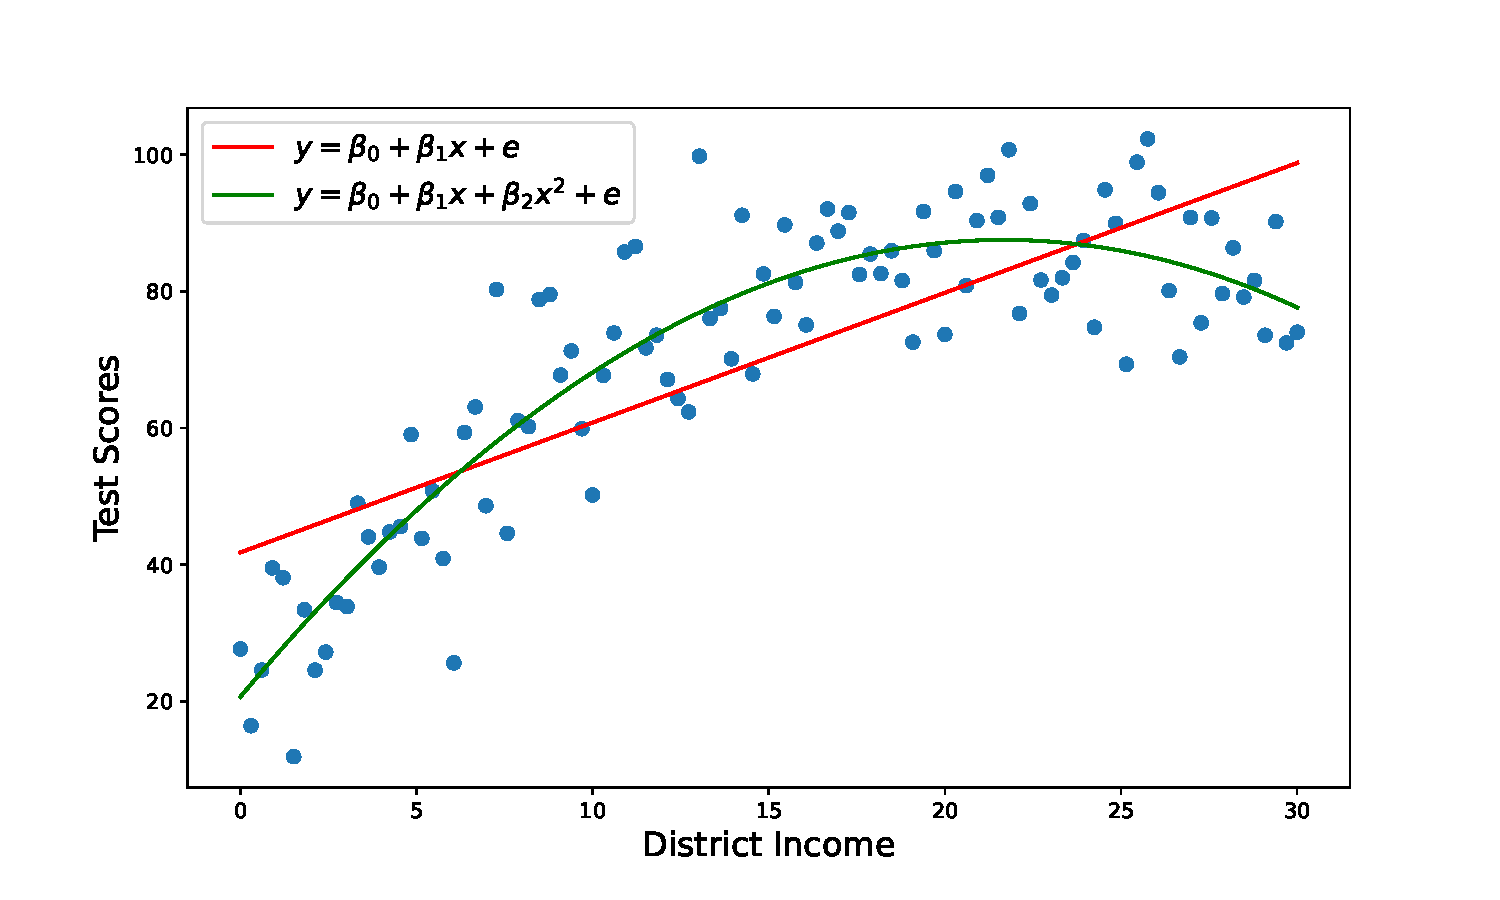
\includegraphics[width=0.8\linewidth]{figures/quadratic_regression.pdf}
                \caption{Linear and quadratic regression}
                \label{fig:research/spec/quad}
            \end{figure}
            Is this a limitation of the linear regression model? Not necessarily. In most cases, we can modify the regressor to be a non-linear function of $x$; for example, consider the log-linear regression model of $y$ on $\log x$,
            \begin{align}
                y_i = \beta_0 + \beta_1 \log x_i + u_i
            \end{align}
            We consider two main types of functional form: polynomial (quadratic) and logarithmic types, and discuss the \textbf{interpretation} of the coefficients.

            \begin{definition}[Quadratic spec.]
                The \textit{quadratic linear regression} takes the form
                \begin{align}
                    y_i = \beta_0 + \beta_1 x + \beta_2 x^2 + u_i
                \end{align}
            \end{definition}


            \begin{definition}[Linear-log spec.]
                The \textit{linear-log regression} takes the form
                \begin{align}
                    y_i = \beta_0 + \beta_1 \log x_i + u_i
                \end{align}
            \end{definition}
            \begin{lemma}
                In a linear-log regression, a local change in $x_i$ by 1\% approximately changes $y_i$ by $0.01\beta_1$
            \end{lemma}
            \begin{proof}
                By the chain rule, 
                \begin{align*}
                    \Delta y
                        &= \odv{y}{x}\Delta x \\
                        &= \odv{y}{\log x}\odv{\log x}{x}\Delta x\\  
                        &= \beta_1\frac{\Delta x}{x}    
                \end{align*}
                Thus if $x$ increases by 1\%, then $\Delta x/x = 0.01$, and $\Delta y = 0.01\,\beta_1$.
            \end{proof}
            
            In addition, we can transform the outcome variable $y$.
            \begin{definition}[Log-linear spec.]
                The \textit{log-linear regression} takes the form
                \begin{align}
                    \log y_i = \beta_0 + \beta_1 x_i + u_i
                \end{align}
            \end{definition}
            \begin{lemma}
                In a log-linear regression, a local change in $x_i$ by 1 unit approximately changes $y_i$ by $100\,\beta_1$\%.
            \end{lemma}
            \begin{proof}
                By the chain rule, 
                \begin{align*}
                    \Delta y
                        &= \odv{y}{x}\Delta x \\
                        &= \odv{y}{\log y}\odv{\log y}{x}\Delta x\\  
                        &= y\beta_1\Delta x    
                \end{align*}
                which implies
                \begin{align}
                    \frac{\Delta y}{y} = \beta_1\Delta x
                \end{align}
                Thus if $\Delta x = 1$, then $\Delta y/y = \beta_1$, and so $y$ increases by $100\,\beta_1$\%.
            \end{proof}

            
            \begin{definition}[Log-log spec.]
                The \textit{log-log regression} takes the form
                \begin{align}
                    \log y_i = \beta_0 + \beta_1 \log x_i + u_i
                \end{align}
            \end{definition}
            \begin{lemma}
                In a log-log regression, a local change in $x_i$ by 1\% approximately changes $y_i$ by $\beta_1$\%. We call $\beta_1$ the \textit{elasticity}.
            \end{lemma}
            \begin{proof}
                By the chain rule, 
                \begin{align*}
                    \frac{\Delta y}{y}
                        &= \frac{1}{y}\odv{y}{x}\Delta x \\
                        &= \frac{1}{y}\odv{y}{\log y}\odv{\log y}{\log x}\odv{\log x}{x}\Delta x    \\
                        &= \beta_1 \frac{\Delta x}{x}
                \end{align*}
                Thus if $x$ locally increases by 1\%, that is $\Delta x/x = 0.01$, then $\Delta y/y = \beta_1$, and so $y$ increases by $\beta_1$\%.
            \end{proof}

            
        \subsection{Standardising variables}
            Another choice we can make is to standardise our variables. Consider the regression model,
            \begin{align}
                y = \beta_0 + \beta_1 x + u
            \end{align}
            We can
            \begin{enumerate}
                \item \textbf{standardise} $x$; define
                \begin{align}
                    x_i^* := \frac{x_i-\mu_x}{\sigma_x} 
                \end{align}
                and specifying the model as
                \begin{align}
                    y_i  = \beta_0^* + \beta_1^* x^*_i+u_i^*
                \end{align}
                Now the interpretation of $\beta_1^*$ is the average change in $y$ associated with changing $x$ by one standard deviation.

                \item \textbf{standardise} $y$; define
                \begin{align}
                    y_i^* := \frac{y_i-\mu_y}{\sigma_y} 
                \end{align}
                and specifying the model as
                \begin{align}
                    y_i ^* = \beta_0^*+\beta_1^* x_i+u_i^*
                \end{align}
                Now the interpretation of $\beta_1^*$ is the average change in $y^*$ associated with changing $x$ by one. A change in $y^*$ by one is a change in $y$ by one standard deviation.

                \item \textbf{standardise both}; define $x^*$ and $y^*$ as above, then specify the model as
                \begin{align}
                    y_i ^* = \beta_0^*+\beta_1^* x^*_i+u_i^*
                \end{align}
                As standard, $\beta_1^*$ is interpreted as `the average change in $y^*$ that is associated with $x^*$ increasing by 1'. However, due to normalising, this is “the average number of standard deviations that $y$ changes by that is associated with $x$ increasing by one standard deviation.
            \end{enumerate}

            We have multiple ways to implement this in STATA; see Listing \ref{lst:research/standardise}.

            \begin{sexylisting}[colback=white, label=lst:research/standardise]{Standardising variables}
//  Method 1:

//  Run a summary first:
    sum x

//  Generate variables
    gen x_full_std = (x - r(mean))/r(sd)

//  Method 2:

//  Use egen and std
    egen x_full_std = std(x)
            \end{sexylisting}
            
            

        
        

        
        
            
\chapter{Endogeneity}

    To ensure unbiasedness of OLS estimator, or at least consistency of the OLS estimator we need to have \textit{exogeneity} of the errors, that is
    \begin{align}
        \cov{x,u} = 0
    \end{align}
    The failure of this assumption is called \textit{endogeneity}. Endogeneity can arise for a number of reasons:
    \begin{itemize}
        \item omitted variables
        \item lagged $y$ in the presence of autocorrelation in the error term
        \item simultaneity
        \item measurement errors
    \end{itemize}
    In this chapter we discuss how endogeneity can arise, and several strategies to overcome this.

    \section{Instrumental Variables (IV)}
        
        \subsection{Motivation}

            Suppose we have the following bivariate linear regression model:
            \begin{align}
                y = \beta_0 + \beta_1 x + u
            \end{align}
            If we have endogeneity, i.e. $\cov{x,u} = 0$, then our OLS estimates will be in general, biased. The approach of the previous chapters was to ensure the confounders were appropriately controlled for, and hope $x$ is no longer endogenous. In this section, we introduce another method; through the use of an \textit{instrumental variable} to deal with the endogenous regressor.
            \begin{figure}
                \centering
                
\tikzset{every picture/.style={line width=0.75pt}} %set default line width to 0.75pt        

\begin{tikzpicture}[x=0.75pt,y=0.75pt,yscale=-1,xscale=1]
%uncomment if require: \path (0,524); %set diagram left start at 0, and has height of 524

%Rounded Rect [id:dp6497612275953306] 
\draw   (110,203) .. controls (110,195.82) and (115.82,190) .. (123,190) -- (237,190) .. controls (244.18,190) and (250,195.82) .. (250,203) -- (250,317) .. controls (250,324.18) and (244.18,330) .. (237,330) -- (123,330) .. controls (115.82,330) and (110,324.18) .. (110,317) -- cycle ;

%Rounded Rect [id:dp8673780682403747] 
\draw  [color={rgb, 255:red, 81; green, 179; blue, 2 }  ,draw opacity=1 ][line width=1.5]  (120,108) .. controls (120,103.58) and (123.58,100) .. (128,100) -- (232,100) .. controls (236.42,100) and (240,103.58) .. (240,108) -- (240,132) .. controls (240,136.42) and (236.42,140) .. (232,140) -- (128,140) .. controls (123.58,140) and (120,136.42) .. (120,132) -- cycle ;

%Straight Lines [id:da16218237230483512] 
\draw [color={rgb, 255:red, 208; green, 2; blue, 27 }  ,draw opacity=1 ][line width=1.5]    (240,300) -- (346,300) ;
\draw [shift={(350,300)}, rotate = 180] [fill={rgb, 255:red, 208; green, 2; blue, 27 }  ,fill opacity=1 ][line width=0.08]  [draw opacity=0] (11.61,-5.58) -- (0,0) -- (11.61,5.58) -- cycle    ;
%Straight Lines [id:da880895933850384] 
\draw [color={rgb, 255:red, 81; green, 179; blue, 2 }  ,draw opacity=1 ][line width=1.5]    (180,140) -- (180,196) ;
\draw [shift={(180,200)}, rotate = 270] [fill={rgb, 255:red, 81; green, 179; blue, 2 }  ,fill opacity=1 ][line width=0.08]  [draw opacity=0] (11.61,-5.58) -- (0,0) -- (11.61,5.58) -- cycle    ;
%Straight Lines [id:da6515543213351532] 
\draw [color={rgb, 255:red, 81; green, 179; blue, 2 }  ,draw opacity=1 ][line width=1.5]    (240,220) -- (346,220) ;
\draw [shift={(350,220)}, rotate = 180] [fill={rgb, 255:red, 81; green, 179; blue, 2 }  ,fill opacity=1 ][line width=0.08]  [draw opacity=0] (11.61,-5.58) -- (0,0) -- (11.61,5.58) -- cycle    ;
%Rounded Rect [id:dp3607596248065986] 
\draw  [color={rgb, 255:red, 208; green, 2; blue, 27 }  ,draw opacity=1 ][line width=1.5]  (220,388) .. controls (220,383.58) and (223.58,380) .. (228,380) -- (372,380) .. controls (376.42,380) and (380,383.58) .. (380,388) -- (380,412) .. controls (380,416.42) and (376.42,420) .. (372,420) -- (228,420) .. controls (223.58,420) and (220,416.42) .. (220,412) -- cycle ;

%Straight Lines [id:da11780334258026348] 
\draw [color={rgb, 255:red, 208; green, 2; blue, 27 }  ,draw opacity=1 ][line width=1.5]    (222,382) -- (182.24,323.31) ;
\draw [shift={(180,320)}, rotate = 55.89] [fill={rgb, 255:red, 208; green, 2; blue, 27 }  ,fill opacity=1 ][line width=0.08]  [draw opacity=0] (11.61,-5.58) -- (0,0) -- (11.61,5.58) -- cycle    ;
%Straight Lines [id:da6916433454902036] 
\draw [color={rgb, 255:red, 208; green, 2; blue, 27 }  ,draw opacity=1 ][line width=1.5]    (378,382) -- (417.49,333.11) ;
\draw [shift={(420,330)}, rotate = 128.93] [fill={rgb, 255:red, 208; green, 2; blue, 27 }  ,fill opacity=1 ][line width=0.08]  [draw opacity=0] (11.61,-5.58) -- (0,0) -- (11.61,5.58) -- cycle    ;
%Rounded Rect [id:dp8490775320395935] 
\draw  [color={rgb, 255:red, 208; green, 2; blue, 27 }  ,draw opacity=1 ][line width=1.5]  (120,288) .. controls (120,283.58) and (123.58,280) .. (128,280) -- (232,280) .. controls (236.42,280) and (240,283.58) .. (240,288) -- (240,312) .. controls (240,316.42) and (236.42,320) .. (232,320) -- (128,320) .. controls (123.58,320) and (120,316.42) .. (120,312) -- cycle ;

%Rounded Rect [id:dp9976354424664228] 
\draw   (350,203) .. controls (350,195.82) and (355.82,190) .. (363,190) -- (477,190) .. controls (484.18,190) and (490,195.82) .. (490,203) -- (490,317) .. controls (490,324.18) and (484.18,330) .. (477,330) -- (363,330) .. controls (355.82,330) and (350,324.18) .. (350,317) -- cycle ;

%Rounded Rect [id:dp7868826959222632] 
\draw  [color={rgb, 255:red, 81; green, 179; blue, 2 }  ,draw opacity=1 ][line width=1.5]  (120,208) .. controls (120,203.58) and (123.58,200) .. (128,200) -- (232,200) .. controls (236.42,200) and (240,203.58) .. (240,208) -- (240,232) .. controls (240,236.42) and (236.42,240) .. (232,240) -- (128,240) .. controls (123.58,240) and (120,236.42) .. (120,232) -- cycle ;


% Text Node
\draw (135,208) node [anchor=north west][inner sep=0.75pt]  [font=\scriptsize] [align=left] {\begin{minipage}[lt]{63.85pt}\setlength\topsep{0pt}
\begin{center}
\textcolor[rgb]{0.32,0.7,0.01}{Unbiased variation }\\\textcolor[rgb]{0.32,0.7,0.01}{caused by IV}
\end{center}

\end{minipage}};
% Text Node
\draw (128,288) node [anchor=north west][inner sep=0.75pt]  [font=\scriptsize] [align=left] {\begin{minipage}[lt]{72.98pt}\setlength\topsep{0pt}
\begin{center}
\textcolor[rgb]{0.82,0.01,0.11}{Biased variation }\\\textcolor[rgb]{0.82,0.01,0.11}{caused by confounder}
\end{center}

\end{minipage}};
% Text Node
\draw (158,113.4) node [anchor=north west][inner sep=0.75pt]    {$\textcolor[rgb]{0.32,0.7,0.01}{Z_{i} \ \text{(IV)}}$};
% Text Node
\draw (255,393.4) node [anchor=north west][inner sep=0.75pt]    {$\textcolor[rgb]{0.82,0.01,0.11}{W_{i} \ \text{(confounder)}}$};
% Text Node
\draw (385,252.4) node [anchor=north west][inner sep=0.75pt]    {$Y_{i} \ \text{(outcome)}$};
% Text Node
\draw (143,251.4) node [anchor=north west][inner sep=0.75pt]    {$D_{i} \ \text{(treatment)}$};


\end{tikzpicture}
                \caption{Mechanism behind IV}
                \label{fig:IV}
            \end{figure}

            \begin{definition}[IV]
                A valid \textit{instrumental variable}, $z_i$ satisfies two conditions
                \begin{enumerate}
                    \item $z$ is \textbf{exogenous} to the equation, i.e. 
                    \begin{align}
                        \cov{z,u} = 0
                    \end{align}
                    \item $z$ is \textbf{relevant} for explaining $x$, i.e.
                    \begin{align}
                        \cov{z,x} = 0
                    \end{align}
                \end{enumerate}
            \end{definition}

        \subsection{Estimator derivation}
            \begin{theorem}
                If $z$ is an instrumental variable, then $\beta$ can be recovered through
                \begin{align}
                    \beta = \frac{\cov{z,y}}{\cov{z,x}}
                \end{align}
            \end{theorem}
            \begin{proof}
                We have that
                \begin{align}
                    \operatorname{cov}(z,y)= \operatorname{cov}(z,\beta_0 +\beta_1 x +u ) = \beta_1\operatorname{cov}(z, x)
                \end{align}
                Rearrange to yield the result.
            \end{proof}
            \begin{definition}[IV estimator]
                The IV estimator is the MM estimator of $\beta$,
                \begin{align}
                    \hat\beta^\mathrm{IV}_1 = \frac{\ecov{z,y}}{\ecov{z,x}}
                \end{align}
            \end{definition}
            Why is such an instrument beneficial for estimating $\beta_1$? As we know $x$ could be endogenous, this means it is correlated with unknown confounders, as shown in Figure \ref{fig:IV}, and so OLS will produce biased estimates. A valid instrument will allow us to isolate the variation in  uncorrelated with confounders, we call $\hat x_i$, and estimate the effect of $\hat x_i$ on $y_i$, defined as $\hat\beta^\mathrm{IV}_1$ which is a consistent estimate of $\beta_1$ (although it turns out not unbiased).

        \subsection{Wald estimator}\label{def:endogeneity/Wald}
            \begin{definition}
                The \textit{Wald estimator} is defined as
                \begin{align*}
                    \hat\beta_1^\mathrm{Wald} := \frac{\hat\pi_1}{\hat \delta_1}
                \end{align*}
                where $\hat\delta_j$ are the \textit{first stage} regression coefficients,
                \begin{align}
                    x_i = \delta_0 + \delta_1 z_i + e_i 
                \end{align}
                and $\hat\pi_j$ are the \textit{reduced form} coefficients,
                \begin{align}
                    y_i = \pi_0 + \pi_1 z_i + \nu_i
                \end{align}
            \end{definition}
            
            This is equivalent to the IV estimator defined above as
            \begin{align}
                \hat\beta_1^\mathrm{Wald} = \frac{\frac{\ecov{z,y}}{\evar{z}}}{\frac{\ecov{z,x}}{\evar{z_i}}} = \hat\beta^\mathrm{IV}
            \end{align}

        
    \section{Two Stage Least Squares (2SLS)}
    
        IV allows us to overcome selection bias due to endogeneity. 2SLS allows us to generalise IV to binary, count or continuous variables and augment the equation with controls. In addition we can leverage multiple instruments to improve our estimates.

        \subsection{Motivation}
            Let $x$ be our explanatory variable, $y$ is the outcome variable and $z$ is a valid instrument. A baseline regression model would be
            \begin{align}
                y_i = \beta_0 + \beta_1 x_i + u_i
            \end{align}
            However we know that exogeneity fails for $x$, thus OLS is inconsistent and biased.
            
            Recall with \textit{IV/Wald estimators}, we can overcome this by estimating two equations: `First Stage' and `Reduced Form' models
            \begin{align}
                FS:\quad x_i &= \delta_0 + \delta_1 z_i + e_i\\
                RF:\quad y_i &= \pi_0 + \pi_1 z_i + v_i
            \end{align}
            We then compute the ratio as defined in Definition \ref{def:endogeneity/Wald}.

            \textbf{For 2SLS, we proceed as follows.} 
            \begin{enumerate}
                \item First estimate the first stage
                \begin{align}
                    FS:\quad x_i &= \delta_0 + \delta_1 z_i + e_i
                \end{align}
                and obtain predicted values $\hat x_i = \hat\delta_0 + \hat\delta_1 z_i$.
                
                \item Next, we regress $y_i$ on the predicted value of $x_i$, $\hat x_i$,
                \begin{align}
                    y_i = \beta_0^\mathrm{2SLS} + \beta_1^\mathrm{2SLS} \hat x_i + \varepsilon_i
                \end{align}
            \end{enumerate}


        \subsection{Implementation}
            
            \begin{sexylisting}[colback=white, label=lst:endogeneity/2SLS/implement]{2SLS estimation}
//  Run 2SLS regression (robust): 
//  Syntax: outcome control (endog.vars = instruments), robust
ivregress 2sls y w (x_1 x_2 = z_1 z_2 z_3), robust
            \end{sexylisting}
            \noindent It is important to note we \textit{cannot} do:\\ \\
            \indent\verb|reg x_1 z_1 z_2 z_3 w|    \\
            \indent\verb|predict x_1hat|   \\
            \indent\verb|reg x_2 z_1 z_2 z_3 w|    \\
            \indent\verb|predict x_2hat|   \\
            \indent\verb|reg y x_1hat x_2hat w, robust|\\ \\
            This is because when estimating standard error, STATA computes $\hat u_i$ with $\hat x_{j,i}$ instead of $x_{j,i}$ as defined below:
            \begin{align}
                \hat u_i = y_i - \left(\hat\beta_0^\mathrm{2SLS}+\hat\beta_1^\mathrm{2SLS} x_{1,i}+\hat\beta_2^\mathrm{2SLS}  x_{2,i}+\hat\beta_3^\mathrm{2SLS} w_i\right)
            \end{align}
            
        
    \section{Simultaneous Equation Models (SEM)}

        When we investigate demand and supply, we have two simultaneous equations that determine equilibrium quantity and price.
        
        \subsection{Motivation}
            Since we can only observe the black dots where equilibrium occurs, a regression would lead to a misunderstanding of the model, predicted by the black line. Instead what we want to know are the green and red lines, supply and demand equations.

            \begin{figure}
                \centering
                

\tikzset{every picture/.style={line width=0.75pt}} %set default line width to 0.75pt        

\begin{tikzpicture}[x=0.75pt,y=0.75pt,yscale=-1,xscale=1]
%uncomment if require: \path (0,416); %set diagram left start at 0, and has height of 416

%Shape: Axis 2D [id:dp7232537425646829] 
\draw  (160,270) -- (450,270)(160,70) -- (160,270) -- cycle (443,265) -- (450,270) -- (443,275) (155,77) -- (160,70) -- (165,77)  ;
%Straight Lines [id:da9194583658032972] 
\draw [color={rgb, 255:red, 81; green, 179; blue, 2 }  ,draw opacity=0.55 ] [dash pattern={on 4.5pt off 4.5pt}]  (200,120) -- (340,240) ;
%Straight Lines [id:da09936562819974382] 
\draw [color={rgb, 255:red, 81; green, 179; blue, 2 }  ,draw opacity=0.55 ] [dash pattern={on 4.5pt off 4.5pt}]  (230,100) -- (370,220) ;
%Straight Lines [id:da7284855390717861] 
\draw [color={rgb, 255:red, 81; green, 179; blue, 2 }  ,draw opacity=0.55 ] [dash pattern={on 4.5pt off 4.5pt}]  (260,80) -- (400,200) ;
%Straight Lines [id:da434828806821248] 
\draw [color={rgb, 255:red, 208; green, 2; blue, 27 }  ,draw opacity=0.61 ] [dash pattern={on 4.5pt off 4.5pt}]  (210,200) -- (360,80) ;
%Straight Lines [id:da7067480974690954] 
\draw [color={rgb, 255:red, 208; green, 2; blue, 27 }  ,draw opacity=0.61 ] [dash pattern={on 4.5pt off 4.5pt}]  (240,220) -- (390,100) ;
%Straight Lines [id:da6860399852947346] 
\draw [color={rgb, 255:red, 208; green, 2; blue, 27 }  ,draw opacity=0.61 ] [dash pattern={on 4.5pt off 4.5pt}]  (270,240) -- (420,120) ;
%Flowchart: Connector [id:dp6703726074956241] 
\draw  [fill={rgb, 255:red, 0; green, 0; blue, 0 }  ,fill opacity=1 ] (279.29,143.32) .. controls (279.29,142.59) and (279.89,142) .. (280.64,142) .. controls (281.39,142) and (282,142.59) .. (282,143.32) .. controls (282,144.05) and (281.39,144.64) .. (280.64,144.64) .. controls (279.89,144.64) and (279.29,144.05) .. (279.29,143.32) -- cycle ;
%Flowchart: Connector [id:dp42343723539931355] 
\draw  [fill={rgb, 255:red, 0; green, 0; blue, 0 }  ,fill opacity=1 ] (251,165.68) .. controls (251,164.95) and (251.61,164.36) .. (252.36,164.36) .. controls (253.11,164.36) and (253.71,164.95) .. (253.71,165.68) .. controls (253.71,166.41) and (253.11,167) .. (252.36,167) .. controls (251.61,167) and (251,166.41) .. (251,165.68) -- cycle ;
%Flowchart: Connector [id:dp3602533313351184] 
\draw  [fill={rgb, 255:red, 0; green, 0; blue, 0 }  ,fill opacity=1 ] (305,166.68) .. controls (305,165.95) and (305.61,165.36) .. (306.36,165.36) .. controls (307.11,165.36) and (307.71,165.95) .. (307.71,166.68) .. controls (307.71,167.41) and (307.11,168) .. (306.36,168) .. controls (305.61,168) and (305,167.41) .. (305,166.68) -- cycle ;
%Flowchart: Connector [id:dp5055341802748268] 
\draw  [fill={rgb, 255:red, 0; green, 0; blue, 0 }  ,fill opacity=1 ] (334,143.32) .. controls (334,142.59) and (334.61,142) .. (335.36,142) .. controls (336.11,142) and (336.71,142.59) .. (336.71,143.32) .. controls (336.71,144.05) and (336.11,144.64) .. (335.36,144.64) .. controls (334.61,144.64) and (334,144.05) .. (334,143.32) -- cycle ;
%Flowchart: Connector [id:dp7460489090675402] 
\draw  [fill={rgb, 255:red, 0; green, 0; blue, 0 }  ,fill opacity=1 ] (332,189.68) .. controls (332,188.95) and (332.61,188.36) .. (333.36,188.36) .. controls (334.11,188.36) and (334.71,188.95) .. (334.71,189.68) .. controls (334.71,190.41) and (334.11,191) .. (333.36,191) .. controls (332.61,191) and (332,190.41) .. (332,189.68) -- cycle ;
%Straight Lines [id:da3662864883226279] 
\draw [color={rgb, 255:red, 0; green, 0; blue, 0 }  ,draw opacity=1 ]   (190,130) -- (430,193) ;

% Text Node
\draw (191,72) node [anchor=north west][inner sep=0.75pt]  [color={rgb, 255:red, 81; green, 179; blue, 2 }  ,opacity=1 ] [align=left] {demand};
% Text Node
\draw (381,82) node [anchor=north west][inner sep=0.75pt]  [color={rgb, 255:red, 81; green, 179; blue, 2 }  ,opacity=1 ] [align=left] {\textcolor[rgb]{0.82,0.01,0.11}{supply}};
% Text Node
\draw (410,201) node [anchor=north west][inner sep=0.75pt]   [align=left] {reduced form\\regression};
% Text Node
\draw (135,42.4) node [anchor=north west][inner sep=0.75pt]    {$p,\ \text{price}$};
% Text Node
\draw (411,281.4) node [anchor=north west][inner sep=0.75pt]    {$q,\ \text{quantity}$};


\end{tikzpicture}
                \caption{Simultaneity bias}
                \label{fig:endogeneity/sem}
            \end{figure}

            Now suppose we have the model, or structural equations:
            \begin{align}
                &q_i =\beta_0^{(d)}+\beta_1^{(d)}p_i+e_i^{(d)}\\
                &q_i =\beta_0^{(s)}+\beta_1^{(s)}p_i+e_i^{(s)}
            \end{align}
            We would like to be able to hold one curve constant, while shifting the other, which would allow use to estimate the former, as shown on Figure X. Therefore we need a instrument that will shift one curve and allow us to estimate the other. Let this instrument be denoted $z$, and so our model becomes:
            \begin{align}
                &q_i =\beta_0^{(d)} + \beta_1^{(d)}p_i + e_i^{(d)}\label{eq:endogeneity/demand}\\
                &q_i =\beta_0^{(s)} + \beta_1^{(s)}p_i + \beta_2^{(s)}z^{(s)}_i + e_i^{(s)}\label{eq:endogeneity/supply_w_IV}
            \end{align}
            What properties does this instrument need to satisfy? We assume
            \begin{enumerate}
                \item \textbf{the instrument shifts the curve (i.e. supply curve)} - our relevance condition:
                \begin{align}
                    \cov{z^{(s)}, p} \neq 0
                \end{align}
                
                \item \textbf{the instrument does not move the other curve (i.e. demand curve)} - our exogeneity condition:
                \begin{align}
                    \cov{z^{(s)},e^{(d)}} = 0
                \end{align}
                
                \item \textbf{the instrument does not does not directly affect demand}, only affecting quantity through shifting supply - our exclusion condition.
            \end{enumerate}
            \begin{figure}
                \centering
                

\tikzset{every picture/.style={line width=0.75pt}} %set default line width to 0.75pt        

\begin{tikzpicture}[x=0.75pt,y=0.75pt,yscale=-1,xscale=1]
%uncomment if require: \path (0,416); %set diagram left start at 0, and has height of 416

%Shape: Axis 2D [id:dp7232537425646829] 
\draw  (160,270) -- (450,270)(160,70) -- (160,270) -- cycle (443,265) -- (450,270) -- (443,275) (155,77) -- (160,70) -- (165,77)  ;
%Straight Lines [id:da09936562819974382] 
\draw [color={rgb, 255:red, 81; green, 179; blue, 2 }  ,draw opacity=1 ]   (230.43,100.27) -- (242.29,110.44) -- (393,240) ;
%Straight Lines [id:da434828806821248] 
\draw [color={rgb, 255:red, 208; green, 2; blue, 27 }  ,draw opacity=0.61 ] [dash pattern={on 4.5pt off 4.5pt}]  (182,178) -- (332,58) ;
%Straight Lines [id:da7067480974690954] 
\draw [color={rgb, 255:red, 208; green, 2; blue, 27 }  ,draw opacity=0.61 ] [dash pattern={on 4.5pt off 4.5pt}]  (240,220) -- (390,100) ;
%Straight Lines [id:da6860399852947346] 
\draw [color={rgb, 255:red, 208; green, 2; blue, 27 }  ,draw opacity=0.61 ] [dash pattern={on 4.5pt off 4.5pt}]  (270,240) -- (420,120) ;
%Flowchart: Connector [id:dp6703726074956241] 
\draw  [fill={rgb, 255:red, 0; green, 0; blue, 0 }  ,fill opacity=1 ] (279.29,143.32) .. controls (279.29,142.59) and (279.89,142) .. (280.64,142) .. controls (281.39,142) and (282,142.59) .. (282,143.32) .. controls (282,144.05) and (281.39,144.64) .. (280.64,144.64) .. controls (279.89,144.64) and (279.29,144.05) .. (279.29,143.32) -- cycle ;
%Flowchart: Connector [id:dp42343723539931355] 
\draw  [fill={rgb, 255:red, 0; green, 0; blue, 0 }  ,fill opacity=1 ] (357.29,209.68) .. controls (357.29,208.95) and (357.89,208.36) .. (358.64,208.36) .. controls (359.39,208.36) and (360,208.95) .. (360,209.68) .. controls (360,210.41) and (359.39,211) .. (358.64,211) .. controls (357.89,211) and (357.29,210.41) .. (357.29,209.68) -- cycle ;
%Flowchart: Connector [id:dp3602533313351184] 
\draw  [fill={rgb, 255:red, 0; green, 0; blue, 0 }  ,fill opacity=1 ] (305,166.68) .. controls (305,165.95) and (305.61,165.36) .. (306.36,165.36) .. controls (307.11,165.36) and (307.71,165.95) .. (307.71,166.68) .. controls (307.71,167.41) and (307.11,168) .. (306.36,168) .. controls (305.61,168) and (305,167.41) .. (305,166.68) -- cycle ;
%Flowchart: Connector [id:dp5055341802748268] 
\draw  [fill={rgb, 255:red, 0; green, 0; blue, 0 }  ,fill opacity=1 ] (252,120.32) .. controls (252,119.59) and (252.61,119) .. (253.36,119) .. controls (254.11,119) and (254.71,119.59) .. (254.71,120.32) .. controls (254.71,121.05) and (254.11,121.64) .. (253.36,121.64) .. controls (252.61,121.64) and (252,121.05) .. (252,120.32) -- cycle ;
%Flowchart: Connector [id:dp7460489090675402] 
\draw  [fill={rgb, 255:red, 0; green, 0; blue, 0 }  ,fill opacity=1 ] (332,188.68) .. controls (332,187.95) and (332.61,187.36) .. (333.36,187.36) .. controls (334.11,187.36) and (334.71,187.95) .. (334.71,188.68) .. controls (334.71,189.41) and (334.11,190) .. (333.36,190) .. controls (332.61,190) and (332,189.41) .. (332,188.68) -- cycle ;
%Straight Lines [id:da27407798874237244] 
\draw [color={rgb, 255:red, 208; green, 2; blue, 27 }  ,draw opacity=0.61 ] [dash pattern={on 4.5pt off 4.5pt}]  (210,200) -- (360,80) ;
%Straight Lines [id:da6180788422321196] 
\draw [color={rgb, 255:red, 208; green, 2; blue, 27 }  ,draw opacity=0.61 ] [dash pattern={on 4.5pt off 4.5pt}]  (295,261) -- (445,141) ;

% Text Node
\draw (184,82) node [anchor=north west][inner sep=0.75pt]  [color={rgb, 255:red, 81; green, 179; blue, 2 }  ,opacity=1 ] [align=left] {demand};
% Text Node
\draw (381,82) node [anchor=north west][inner sep=0.75pt]  [color={rgb, 255:red, 81; green, 179; blue, 2 }  ,opacity=1 ] [align=left] {\textcolor[rgb]{0.82,0.01,0.11}{supply}};
% Text Node
\draw (135,42.4) node [anchor=north west][inner sep=0.75pt]    {$p,\ \text{price}$};
% Text Node
\draw (411,281.4) node [anchor=north west][inner sep=0.75pt]    {$q,\ \text{quantity}$};


\end{tikzpicture}
                \caption{Instrument shifting supply curve}
                \label{fig:endogeneity/sem/iv}
            \end{figure}
            

        \subsection{IV estimation}
            Since we have established that  is an instrumental variable, we can estimate  with IV. Recall the definition of the IV estimator:
            \begin{align}
                \hat\beta^{(s),IV}_1 = \frac{\ecov{z^{(s)},q}}{\ecov{z^{(s)},p}}
            \end{align}
            We can implement this in STATA by performing the 2SLS method,
            \begin{itemize}
                \item \textbf{First stage.} Estimate the regression
                \begin{align}
                    p_i = \pi_0 + \pi_1 z_i^{(s)} + e_i
                \end{align}
                and obtaining the estimate $\hat p_i = \hat\pi_0 + \hat\pi_1 z_i^{(s)}$.

                \item \textbf{Second stage.} Estimate the regression
                \begin{align}
                    q_i = \beta_0^{(d)} + \beta_1^{(d)} \hat p_i + u_i^{(d)}
                \end{align}
            \end{itemize}
            
            To implement in STATA, refer to the code in Lising \ref{lst:endogeneity/SEM/2SLS}.
            \begin{sexylisting}[colback=white, label=lst:endogeneity/SEM/2SLS]{2SLS SEM estimation}
ivregress 2sls qty (price = supply_shift), robust
            \end{sexylisting}

            
        \subsection{Reduced form estimation}

            We know that in equilibrium, demand is equal to supply, therefore setting \eqref{eq:endogeneity/demand} equal to \eqref{eq:endogeneity/supply_w_IV}, by 
            \begin{itemize}
                \item \textbf{equating} $q_i$, we obtain
                \begin{align}
                    \beta_0^{(d)} + \beta_1^{(d)}p_i + e_i^{(d)} = \beta_0^{(s)} + \beta_1^{(s)}p_i + \beta_2^{(s)}z^{(s)}_i + e_i^{(s)}
                \end{align}
                which rearranges to yield
                \begin{align}
                    p_i = \pi_0 + \pi_1 z_i^{(s)} + e_i
                \end{align}
                where
                \begin{align}
                    \delta_0 := \frac{\beta_0^{(s)} - \beta_0^{(d)}}{\beta_1^{(d)} - \beta_1^{(s)}},\quad \delta_1 := \frac{\beta_2^{(s)} - \beta_0^{(d)}}{\beta_1^{(d)} - \beta_1^{(s)}},\quad e_i := \frac{u_i^{(s)}-u_i^{(d)}}{\beta_1^{(d)} - \beta_1^{(s)}}
                \end{align}

                \item \textbf{equating} $p_i$ (first rearranging \eqref{eq:endogeneity/demand} and \eqref{eq:endogeneity/supply_w_IV} for $p_i$), it can be shown that 
                \begin{align}
                    q_i = \pi_0 +\pi_1 z_i^{(s)} + v_i
                \end{align}
                where
                \begin{align}
                    \pi_0 := \beta_0^{(d)},\quad\pi_1 := \frac{\beta_1^{(d)}\beta_2^{(s)}}{\beta_1^{(d)} - \beta_1^{(s)}},\quad v_i = \frac{\beta_1^{(d)}u_i^{(s)} - \beta_1^{(s)}u_i^{(d)}}{\beta_1^{(d)} - \beta_1^{(s)}}
                \end{align}
            \end{itemize}
            Therefore, we note that the ratio of the coefficients gives $\beta_1^{(d)}$, more precisely,
            \begin{align}
                \beta_1^{(d)} = \frac{\pi_1}{\delta_1}
            \end{align}
            There we have it - if we estimate the two reduced form equations, then we can estimate the demand curve slope.

\chapter{Panel Data Methods}
	\begin{definition}[Panel data]
		Panel data is cross-sectional data, observed over time for each individual.
	\end{definition}
	An example of such data is the multivariate linear regression model given by
	\begin{align}
		y_{it} = \beta_0 +\beta_1 x_{1,it}+\dots +\beta_k x_{k,it}+u_{it}
	\end{align}
	where $i=1,2,\dots,n$ indexes individuals, while $t=1,2\dots,T$ simultaneously indexes the observation time for individual $i$.
	
	Another seemingly similar type of data is called \textit{repeated cross section}; note this is not the same a panel data, as it does not necessarily hold that the same individuals are observed over time.
	
	For panel data, in general we can decompose the error term $u_i$ into a time-invariant component $a_i$ and a de-trended error, $v_{it}$,
	\begin{align}
		y_{it} = \beta_0 +\beta_1 x_{1,it}+ \cdots +\beta_k x_{k,it} +a_i +v_{it}
	\end{align}
	$a_i$ represents the `effect of being individual $i$'. A big problem for us econometricians is that $a_i$ can be highly correlated with our regressors, and hence induce bias. Although this problem is not unique to panel data, the nature/strength of panel data allows us to overcome this issue. We will two major estimators:
	\begin{enumerate}
		\item \textbf{First Differences (FD)}
		\item \textbf{Fixed Effects (FE)}
	\end{enumerate}
	In this chapter we will also discuss the Difference-in-Differences (DiD) estimator, a method to deal with before and after treatment data with two groups - a specific kind of panel data.
	
    \section{First Differences (FD)}
        \subsection{Estimator derivation}
            Define $\Delta y_{it} = y_{it} - y_{i(t-1)}$ as the change in the outcome variable over time for individual $i$.
            \begin{definition}[First differences estimator]
                Assuming the linear regression model, the \textit{First Differences} (FD) estimator, is the OLS estimator of the regression model (without constant):
    			\begin{align}
    				\Delta y_{it} = \beta_1 \Delta x_{1,it} + \dots +\beta_k \Delta x_{k,it} + \Delta v_{it}
    			\end{align}
    			where $\Delta x_{j,it} = x_{j,it} - x_{j,i(t-1)}$.
    		\end{definition}
    		\begin{proof}
    			Assuming the linear regression model, we have
    			\begin{align*}
    				\Delta y_{it}
    		      		&:=  y_{it} - y_{i,t-1}\\
    					&= \left(\beta_0 +\beta_1 x_{1,it}+\cdots+\beta_k x_{k,it} +a_i +v_{it}\right) \\
    					&\phantom{-}\qquad- \left(\beta_0 +\beta_1 x_{1,i(t-1)}+ \cdots +\beta_k x_{k,i(t-1)} +a_i +v_{i(t-1)}\right)\\
    					&= 
    					(\beta_0-\beta_0 ) + (\beta_1x_{1,it}-\beta_1x_{1,i(t-1)} ) +\\
    					&\phantom{=}\qquad\dots+ (\beta_k x_{k,it}-\beta_k x_{k,i(t-1)} ) +(a_i-a_i)+(v_{it}-v_{i(t-1)}) \\
    					&= \beta_1 \Delta x_{1,it} + \dots +\beta_k \Delta x_{k,it} + \Delta v_{it}
                \end{align*}
            \end{proof}
            
            Note the individual level effect is differenced out, as well as the intercept. Also note we lose the first observation for each $i$. Also note any variable which are time invariant, i.e. don’t change over time, are also differenced out, e.g. blood type.
            
		\subsection{Implementation}
			To summarise the previous section, we first
			\begin{enumerate}[(1)]
				\item calculate the first difference, that is $\{\Delta y_{it}, \Delta x_{1,it} ,\dots ,\Delta x_{k,it}\}$
				\item estimate via OLS with no constant
			\end{enumerate}
			To implement this in STATA, refer to Listing \ref{lst:panel/FD/implement}
			\begin{sexylisting}[colback=white, label=lst:panel/FD/implement]{First Differences Estimator}
//	(setup) Tell STATA we have panel data
	xtset id time

//	(setup) Sort the data by id and time
	sort id time

//	(1) Create differences variables
	gen diff_y = d.y
	gen diff_x_1 = d.x_1
	gen diff_x_2 = d.x_2

//	(2) Run the regression with no constant (nocons)
	reg diff_y diff_x_1 diff_x_2, robust nocons
			\end{sexylisting}
			
		\section{Fixed Effects (FE)}
			\subsection{Estimator derivation}
				To derive the FE estimator, we first demean the data across time, for each individual. Let $\tilde y_{it} := y_{it} - \bar y_{i}, \tilde x_{j,it} = x_{j,it}-\bar x_{j,i}$ and $\tilde v_{it} = v_{it}-\bar v_i$. Any variable that doesn’t change over time becomes 0 after being demeaned, for example $\tilde a_i = 0$, and so we cannot estimate their effect. 
				
				\begin{definition}
					The \textit{fixed effects }estimator is defined the OLS estimator of the regression model
					\begin{align}
						\tilde y_{it} = \beta_1\tilde x_{1,it}+\dots \beta_k\tilde x_{k,it} + \tilde u_{it}
					\end{align}
				\end{definition}
				This method is quite \textit{tedious} so thankfully there is an alternative method, involving dummy variables.
				
			\subsection{Dummy variable implementation}
				Rather than demean every variable, we can instead introduce a dummy variable for all but one of the individuals (to avoid dummy variable trap). Therefore we estimate
				\begin{align}
					\textstyle y_{it} = \beta_0 +\beta_1 x_{1,it}+\dots +\beta_k x_{k,it} +\sum_{i=1}^{n-1}a_i\delta_i +v_{it}
				\end{align}
				
				\noindent\textbf{Interpretation.} How can we interpret the value of $a_i$? It is the average difference in $y_i$ for being associated with individual $i$, compared to the excluded individual, called the `fixed effect'.
				
				In STATA, we implement this as in Listing \ref{lst:panel/FE/dummy}
				\begin{sexylisting}[colback=white, label=lst:panel/FE/dummy]{Fixed Effects Estimator}
//	(setup) Tell STATA we have panel data
	xtset id time

//	(setup) Sort the data by id and time
	sort id time

//	There are two ways to run the regression.
//	xtreg is more elegant, 
//	but we present the other way for completeness.

//	Option 1: Run the regression with xtreg and fe
	xtreg y x_1 x_2 , fe

//	Option 2: Run the regression normally
	xi: reg y x_1 x_2  i.id,
				\end{sexylisting}
				
			\subsection{Time fixed effects}
				We can extend the individual fixed effect to time fixed effects, i.e. the effect of being in a particular time period. We can interpret time and individual fixed effects
				\begin{align}
					\textstyle y_{it} = \beta_0 + \sum_{j=1}^k \beta_j x_{j,it}+\sum_{i=1}^{n-1}a_i\delta_i +\sum_{t=1}^{T-1}c_t\gamma_t+v_{it}
				\end{align}
				where $c_t$ is the effect of being in period $t$, and $\gamma$ is the dummy for time $t$.
				
				In STATA this is peformed as in Listing \ref{lst:panel/FE/dummy_time}
				\begin{sexylisting}[colback=white, label=lst:panel/FE/dummy_time]{FE estimator with time fixed effects}
//	(setup) Tell STATA we have panel data 
	xtset id time

//	(setup) Sort the data by id and time
	sort id time

//	Option 1: Run the regression with xtreg and fe
	xtreg y x_1 x_2 i.time, fe

//	Option 2: Run the regression normally
	xi: reg y x_1 x_2 i.id i.time,
				\end{sexylisting}
				
		\section{Comparison of FE and FD}
			Fixed effects estimation allows us to measure the `fixed effects' and compare them, whereas first differences already difference them out. It turns out that fixed effects is more commonly used due to `simplicity' to implement and the benefits of estimating `fixed effects'. Some additional facts to note that are not examined are:
			\begin{itemize}
				\item The estimators are identical if $T=2$.
				\item FD has smaller variance if the error is a random walk, $u_it = u_{i(t-1)} + \varepsilon_{it}$, but larger if $u_{it}$ is independent.
				\item FD requires weaker technical assumptions for consistency: $\forall j\leq k,t\leq T,  \ \cov{\Delta u_{it},\Delta x_{j,it}} = 0$ and for FE: $\forall j\leq k,t\leq T,s\leq T,  \ \cov{\Delta u_{is},\Delta x_{j,it}}=0$
			\end{itemize}
			In summary, with panel data \textbf{the default strategy should be to estimate a fixed effects model and include time fixed effects}. However, depending on the conditions of the error term, the first difference estimator can be superior especially if the number of time periods is small.
			
    \section{Difference-in-Differences (DiD)}
        The ideal method to estimate a treatment effect is in a randomised trial. Economists rarely have the luxury of running experiments, and we must make use of observational data to estimate treatment effects. Difference-in-differences is a common attempt to create unbiased estimates.
        
        We first set up the model in which DiD is applied. Consistent with notation throughout the book, let $D_{it}$ be a dummy variable denoting treatment. In addition, we assume we have two time periods, $t= 0,1$, where $t=0$ corresponds to pre-treatment, and $t=1$ is post-treatment. Note this is without loss of generality as we can define $t$ as an indicator/dummy variable of $s$ which records the actual time; for instance $t = \ind_{s\geq\theta}$ if treatment occurs in period $\theta$. Let $T,C$ be the set of individuals in treated and control groups respectively.


        \subsection{Estimator derivation}
            Suppose we have the model
			\begin{align}
				y_{it} = \delta D_{it} + \gamma_i + \lambda_t + v_{it}
			\end{align}
			where $\delta$ is the effect of treatment, $\gamma_i$ controls for the group (treatment/control) taking values $\gamma_C,\gamma_T$  and $\lambda_t$ controls for the time period (pre/post). The dummy is slightly modified and takes the form
			\begin{align}
				D_{it} =
				\begin{cases}
					1 & \text{if }i\in T\text{ and } t=1\\
					0 & \text{otherwise}
				\end{cases}
			\end{align}

            \begin{definition}[DiD estimator]
                The \textit{Difference-in-Differences} (DiD) estimator is defined as
                \begin{align}
                    \hat\delta_\text{DiD}
                        &= \left(\bar y_\text{post}^\text{treat}-\bar y_\text{pre}^\text{treat}\right)-\left(\bar y_\text{post}^\text{control}-\bar y_\text{post}^\text{control}\right)\\
                        &=\sum_{i\in T} (y_{i1} - y_{i0}) - \sum_{i\in C} (y_{i1} - y_{i0})
                \end{align}
                It is called difference-in-difference as we take the difference in outcomes over time, then difference the change in outcome between the two groups.
            \end{definition}
            \begin{proof}
                For
                \begin{itemize}
                    \item \textbf{control group, $i\in C$}
                    \begin{align}
                        & y_{i0} = \gamma_C + \lambda_0 + v_{i0}   \\
                        & y_{i1} = \gamma_C + \lambda_1 + v_{i1}   
                    \end{align}
                    \item \textbf{treatment group, $i\in T$}
                    \begin{align}
                        & y_{i0} = \gamma_T + \lambda_0 + v_{i0}   \\
                        & y_{i1} = \delta + \gamma_T + \lambda_1 + v_{i1}   
                    \end{align}
                \end{itemize}
                We would like to know $\delta$. Consider
                \begin{align}
                    (y_{i1} - y_{i0})\ind_{i\in T} - (y_{i1} - y_{i0})\ind_{i\in C}
                        &= \left[(\delta + \gamma_T + \lambda_1 + v_{i1})- (\gamma_T + \lambda_0 + v_{i0})\right]\ind_{i\in T}\nonumber\\
                        &\phantom{=}\qquad  - \left[(\gamma_C + \lambda_1 + v_{i1}) - (\gamma_C + \lambda_0 + v_{i0})\right]\ind_{i\in C}     \\
                        &= \delta + (v_{i1} - v_{i0})\ind_{i\in T} - (v_{i1} - v_{i0})\ind_{i\in C}
                \end{align}
                Taking expectations yields
                \begin{align}
                    \expect{(y_{i1} - y_{i0})\ind_{i\in T} - (y_{i1} - y_{i0})\ind_{i\in C}} = \delta
                \end{align}
                The DiD estimator is therefore the MM estimator of the above expression.
            \end{proof}

        \subsection{Regression representation}
            We can represent the above in a regression with dummy variables as follows. Keeping the same notation, we have
            \begin{align}
                y_{it} = \beta_0 +\beta_1 t + \beta_2 \ind_{i\in T} + \beta_{3}(t\cdot \ind_{i\in T}) + v_{it}
            \end{align}
            where $\beta_1$ is the difference in being in period post vs pre, $\beta_2$ is the difference just for being in the treated group, and $\beta_3$ is the identified treatment effect.

        \subsection{Implementation}
            To implement DiD in STATA refer to Listing \ref{lst:panel/DiD/implement}.
            \begin{sexylisting}[colback=white, label=lst:panel/DiD/implement]{DiD estimator}
//  Split the data into pre and post (year is the cutoff)
    gen post = time >= year

//  Define the treated dummy and the interaction term
    gen treat = id == treated
    gen treat_post = post * treat

//  Run the DiD regression
    reg y treat post treat_post, robust
            \end{sexylisting}

        \subsection{Parallel trends}
            The important assumption underlying DiD is called ‘parallel trends’ or the effect of time, i.e. $\lambda_1 - \lambda_0$ is equal in both treated and control groups.

            In Figure \ref{fig:panel/DiD/parallel_trend}, we can see that the assumption of parallel trends in the regression representation means that $\beta_1$ lifts both the red and green line. If parallel trends was not true and there was no time effect on the treated group, dotted/red line would be flat.

            \begin{figure}
                \centering
                

\tikzset{every picture/.style={line width=0.75pt}} %set default line width to 0.75pt        

\begin{tikzpicture}[x=0.75pt,y=0.75pt,yscale=-1,xscale=1]
%uncomment if require: \path (0,466); %set diagram left start at 0, and has height of 466

%Shape: Axis 2D [id:dp8173979251061212] 
\draw  (200,320) -- (560,320)(200,70) -- (200,320) -- cycle (553,315) -- (560,320) -- (553,325) (195,77) -- (200,70) -- (205,77)  ;
%Straight Lines [id:da6661208351165583] 
\draw  [dash pattern={on 0.84pt off 2.51pt}]  (360,80) -- (360,320) ;
%Straight Lines [id:da9496708268405148] 
\draw [color={rgb, 255:red, 81; green, 179; blue, 2 }  ,draw opacity=1 ]   (252.31,259.58) -- (467.69,220.42) ;
\draw [shift={(470,220)}, rotate = 349.7] [color={rgb, 255:red, 81; green, 179; blue, 2 }  ,draw opacity=1 ][line width=0.75]      (0, 0) circle [x radius= 3.35, y radius= 3.35]   ;
\draw [shift={(250,260)}, rotate = 349.7] [color={rgb, 255:red, 81; green, 179; blue, 2 }  ,draw opacity=1 ][line width=0.75]      (0, 0) circle [x radius= 3.35, y radius= 3.35]   ;
%Straight Lines [id:da7605028786786207] 
\draw [color={rgb, 255:red, 208; green, 2; blue, 27 }  ,draw opacity=1 ]   (252.31,199.58) -- (360,180) ;
\draw [shift={(250,200)}, rotate = 349.7] [color={rgb, 255:red, 208; green, 2; blue, 27 }  ,draw opacity=1 ][line width=0.75]      (0, 0) circle [x radius= 3.35, y radius= 3.35]   ;
%Straight Lines [id:da6204156956628457] 
\draw [color={rgb, 255:red, 208; green, 2; blue, 27 }  ,draw opacity=1 ]   (468.1,101.38) -- (360,180) ;
\draw [shift={(470,100)}, rotate = 143.97] [color={rgb, 255:red, 208; green, 2; blue, 27 }  ,draw opacity=1 ][line width=0.75]      (0, 0) circle [x radius= 3.35, y radius= 3.35]   ;
%Straight Lines [id:da7633688703424713] 
\draw [color={rgb, 255:red, 208; green, 2; blue, 27 }  ,draw opacity=1 ] [dash pattern={on 4.5pt off 4.5pt}]  (470,160) -- (360,180) ;
%Straight Lines [id:da8118050967929765] 
\draw  [dash pattern={on 4.5pt off 4.5pt}]  (200,260) -- (470,260) ;
%Straight Lines [id:da5126836868598805] 
\draw    (500,262) -- (500,317) ;
\draw [shift={(500,317)}, rotate = 270] [color={rgb, 255:red, 0; green, 0; blue, 0 }  ][line width=0.75]    (0,5.59) -- (0,-5.59)   ;
\draw [shift={(500,262)}, rotate = 270] [color={rgb, 255:red, 0; green, 0; blue, 0 }  ][line width=0.75]    (0,5.59) -- (0,-5.59)   ;

%Straight Lines [id:da3500991397548453] 
\draw    (500,222) -- (500,258) ;
\draw [shift={(500,258)}, rotate = 270] [color={rgb, 255:red, 0; green, 0; blue, 0 }  ][line width=0.75]    (0,5.59) -- (0,-5.59)   ;
\draw [shift={(500,222)}, rotate = 270] [color={rgb, 255:red, 0; green, 0; blue, 0 }  ][line width=0.75]    (0,5.59) -- (0,-5.59)   ;

%Straight Lines [id:da4371401624287816] 
\draw    (500,162) -- (500,218) ;
\draw [shift={(500,218)}, rotate = 270] [color={rgb, 255:red, 0; green, 0; blue, 0 }  ][line width=0.75]    (0,5.59) -- (0,-5.59)   ;
\draw [shift={(500,162)}, rotate = 270] [color={rgb, 255:red, 0; green, 0; blue, 0 }  ][line width=0.75]    (0,5.59) -- (0,-5.59)   ;

%Straight Lines [id:da35598018492557226] 
\draw    (500,100) -- (500,158) ;
\draw [shift={(500,158)}, rotate = 270] [color={rgb, 255:red, 0; green, 0; blue, 0 }  ][line width=0.75]    (0,5.59) -- (0,-5.59)   ;
\draw [shift={(500,100)}, rotate = 270] [color={rgb, 255:red, 0; green, 0; blue, 0 }  ][line width=0.75]    (0,5.59) -- (0,-5.59)   ;

%Straight Lines [id:da32753381874785703] 
\draw  [dash pattern={on 0.84pt off 2.51pt}]  (470,100) -- (470,320) ;
\draw [shift={(470,320)}, rotate = 90] [color={rgb, 255:red, 0; green, 0; blue, 0 }  ][fill={rgb, 255:red, 0; green, 0; blue, 0 }  ][line width=0.75]      (0, 0) circle [x radius= 3.35, y radius= 3.35]   ;
%Straight Lines [id:da9408422259752088] 
\draw  [dash pattern={on 0.84pt off 2.51pt}]  (250,200) -- (250,320) ;
\draw [shift={(250,320)}, rotate = 90] [color={rgb, 255:red, 0; green, 0; blue, 0 }  ][fill={rgb, 255:red, 0; green, 0; blue, 0 }  ][line width=0.75]      (0, 0) circle [x radius= 3.35, y radius= 3.35]   ;

% Text Node
\draw (181,331.4) node [anchor=north west][inner sep=0.75pt]    {$\text{pre-treatment, } t=0$};
% Text Node
\draw (401,331.4) node [anchor=north west][inner sep=0.75pt]    {$\text{post-treatment, } t=1$};
% Text Node
\draw (511,120.4) node [anchor=north west][inner sep=0.75pt]    {$\beta _{3}$};
% Text Node
\draw (511,181.4) node [anchor=north west][inner sep=0.75pt]    {$\beta _{2}$};
% Text Node
\draw (512,231.4) node [anchor=north west][inner sep=0.75pt]    {$\beta _{1}$};
% Text Node
\draw (512,281.4) node [anchor=north west][inner sep=0.75pt]    {$\beta _{0}$};
% Text Node
\draw (141,42) node [anchor=north west][inner sep=0.75pt]   [align=left] {expected outcome};


\end{tikzpicture}
                \caption{Parallel trends and DiD}
                \label{fig:panel/DiD/parallel_trend}
            \end{figure}

            How can we test for parallel trends? Although we cannot prove parallel trends holds in our data, we can look at historical data for the two groups, before treatment was applied to see it parallel trends holds. We can run
            \begin{align}
                y_{it} = \gamma_0 + \gamma_1 t + \gamma_2 \ind_{i\in T} + \gamma_3(t\cdot\ind_{i\in T}) + v_{it}
            \end{align}
            on data prior to the cutoff. As $\gamma_3$ represents the additional effect of time on the treated group, we test the hypothesis that $\beta_3 = 0$. If the hypothesis holds, then parallel trends \textbf{is not} violated; this does not prove parallel trends actually holds, only that it is not disproved.

            To do this in STATA, refer to Listing \ref{lst:panel/DiD/parallel_trends}.
            \begin{sexylisting}[colback=white, label=lst:panel/DiD/parallel_trends]{Testing for Parallel Trends}
//  Create the interaction term
    gen treat_time = treat * time

//  Run the regression for time smaller than a cutoff, 
//  labelled year.
    reg y time treat treat_time , robust , if time < year 

//  Use the regression output to see if beta_3 is significantly
//  different from 0.
            \end{sexylisting}

\chapter{Further Identification Methods}
    \section{Regression Discontinuity Design (RDD)}
        The method exploits a setup in which treatment is based on another variable being above or below a threshold. We can exploit this to create a situation in which treatment is as good as assigned.

    	In particular, RDD is a powerful tool as it creates beautiful and convincing graphs. Showing the effect of  on  can be difficult to communicate to all audiences due to the numerous considerations in applied econometric analysis. Hence convincing graphs are important to convey and communicate results to others.

        \subsection{Regression}
            Let $x_i$ be the `running variable', and $D_i$ be a dummy variable constructed by
            \begin{align}
                D_i =
                \begin{cases}
                    1 &\text{if }x_{i} \geq \theta   \\
                    0 &\text{if }x_{i} < \theta
                \end{cases}
            \end{align}
            where $\theta$ is the threshold.

            Examples of this could be: scholarships awarded if test scores $\geq d$; parliamentary majorities, such as seats $\geq 326$ in the UK House of Commons.

            We want to know the effect of being over the threshold, i.e. $D_i$ on $y_i$. Consider the regression,
            \begin{align}
                y_i = \beta_0 +\beta_1 (x_i-\theta) + \beta_2 D_i + \beta_3 (x_i-\theta)\cdot D_i+u_i
            \end{align}
            The regression model in \eqref{eq:} is plotted in Figure XX.
            \begin{figure}
                \centering
                \caption{Caption}
                \label{fig:enter-label}
            \end{figure}

        \subsection{Interpretation}
            How can we interpret the coefficients? To see the meaning behind the regression \eqref{eq:}. we consider the position and slope separately.\\
            
            \noindent\textbf{Intercept and jump.}
            \begin{itemize}
                \item If we are \textit{exactly at the threshold}, that is $x_i = \theta \implies D_i = 1$, then
                \begin{align}
                    \expect{y_i | x_i = \theta} = \beta_0 + \beta_2
                \end{align}
                
                \item If we are \textit{slightly below the threshold}, $x_i = \theta -\varepsilon$ for a very small $\varepsilon>0$, i.e. very close but not equal to $\theta$
                \begin{align}
                    \expect{y_i\lvert x_i = \theta - \varepsilon} \approx \beta_0
                \end{align}
            \end{itemize}\\

            \noindent\textbf{Slopes.}
            \begin{itemize}
                \item If we are \textit{below the threshold}, that is $x_i < \theta\implies D_i=0$, then
                \begin{align}
                    \expect{y_i | x_i < \theta} = \beta_0 + \beta_1 (x_i-\theta)
                \end{align}
                and the slope is
                \begin{align}
                    \pdv*{\expect{y_i|x_i<\theta}}{x_i}= \beta_1
                \end{align}

                \item If we are \textit{above the threshold}, that is $x_i\geq \theta\implies D_i = 1$, then
                \begin{align}
                    \expect{y_i | x_i \geq\theta} = \beta_0 + \beta_1 (x_i-\theta) + \beta_2 + \beta_3 (x_i-\theta)
                \end{align}
                and the slope is
                \begin{align}
                    \pdv*{\expect{y_i|x_i\geq\theta}}{x_i}= \beta_1 + \beta_3
                \end{align}
            \end{itemize}


        \subsection{Motivation and assumptions}
            Let us consider an example. Let $x_i$ be `test scores'`, $D_i$ be a scholarship award and $y_i$ be `years of college received'. We want to know the effect receiving a scholarship may have on years of college completed. A `naive' regression would be
            \begin{align}
                y_i = \beta_0 +\beta_1 x_i +\beta_2 D_i + u_i
            \end{align}
            However, this naive regression can have problems. There are many unobserved characteristics (confounders), such as parent’s income, which may simultaneously affect both $x_i$, test scores and $y_i$, years of college.

            Alternatively, we can use our RDD regression which was
            \begin{align}
                y_i = \beta_0 + \beta_1 (x_i-\theta) + \beta_2 D_i + \beta_3 (x_i-\theta)\cdot D_i + u_i
            \end{align}
            With RDD, we need to restrict our observations to people with similar scores around a window centred at $\theta$. We assume unobserved characteristics of individuals who are slightly above the cutoff, $x_i = \theta + \varepsilon$ are likely to be comparable to unobserved characteristics of individuals slightly below the cutoff, $x_i = \theta - \varepsilon$. In other words, we assume \textbf{confounders remain constant slightly above and below the cutoff}, removing selection bias (see chapter on matching). Since confounders are constant, there is no omitted variable bias and we can interpret the slope statistics as causal.

        \subsection{Implementation}
            The steps to implement RDD involve:
            \begin{enumerate}[(1)]
                \item centering the running variable, i.e. create $x_i-\theta$, 
                \item creating a dummy for the cutoff,
                \item creating the interaction term,
                \item performing the regression.
            \end{enumerate}
            The STATA code to perform steps (1) to (4) is in Listing \ref{lst:RDD}.
            \begin{sexylisting}[colback=white, label=lst:RDD/regression]{RDD}
//  (1) Center the running variable,
    gen x_centered = x - cutoff
    
//  (2) Create a dummy for the cutoff,
    gen treat = x >= cutoff
    
//  (3) Create the interaction term,
    gen interaction = treat * x_centered

//  (4) Run the regression:
    reg y x_centred treat interaction, robust, /*
    */  if inrange(x, min, max)
            \end{sexylisting}

        \subsection{Testing assumptions}
            To summarise what we previously mentioned on assumptions, as we restrict values are close to the cutoff, we assume that confounders between the two groups are constant.

            Importantly, for the RDD assumption to hold true, \textbf{individuals must not be able to choose which side of the cutoff they are on}, and so treatment is as good as random around the cutoff. This is another reason why we only use data around a window of the cutoff to make this assumption believable.

            \begin{example}
                Consider the case that if high school students are awarded `honours' certificate if they read 20 books. Students have the choice if they want to read twenty or more books, and many will read just enough to surpass the cutoff. Therefore treatment will not be as good as randomly assigned at the cutoff.
            \end{example}
            How can we `test' the assumptions? There are two methods to do this:
            \begin{enumerate}
                \item \textbf{Looking at density} - if there are more individuals above than below the cutoff, it is likely that individuals are not as good as randomly assigned, as they are choosing to be one side of the cutoff.
                \item \textbf{Looking at covariate values} - if individuals above and below the cutoff have similar values for observable covariates, then individuals above and below look similar, and treatment is more likely to be as good as random.
            \end{enumerate}
            To implement this in STATA, refer to Listing \ref{lst:RDD_test}
            \begin{sexylisting}[colback=white, label=lst:RDD/test_assumption]{Testing assumptions}
//  (1) Summarise the data above the cutoff. 
//  List controls w_1, w_2 w.r.t. condition: x >= cutoff
    sum w_1 w_2 if x >= cutoff & inrange(x, min, max)
    
//  (2) Summarise the data below the cutoff.
    sum w_1 w_2 if x < cutoff & inrange(x, min, max)

//  For (1), look if the # of observations, Obs, is similar
//  in both tables. For (2), look to see if covariates are
//  similar in value in both tables.
            \end{sexylisting}

        \subsection{Window choice}
            With RDD we have a choice of bandwidth/window. As discussed in before, the small bandwidth helps support our assumption of as good as random assignment near to cutoff. However this reduces the number of observations. Therefore we face a trade-off when choosing our bandwidth size, denoted by \verb|(min, max)| in the code sections before:
            \begin{itemize}
                \item A \textbf{smaller bandwidth} will reduce the number observations, and decrease the precision of our estimates. However, our assumption is more plausible and bias is reduced.
                \item A \textbf{larger bandwidth} will increase the number observations, and increase the precision of our estimates. However, our assumption is less plausible and bias is increased.
            \end{itemize}
            One suggested method to balance the trade-off is to use `Silverman’s rule of thumb', which chooses the bandwidth
            \begin{align}
                \text{Silverman's bandwidth} = 1.06 \hat \sigma_x n^{-\frac{1}{5}}
            \end{align}
            This is derived by minimising mean squared error (MSE), which as mentioned in ST102 is $(\expect{\hat\theta} -\theta )^2 + \var{\hat\theta}$; although we will not prove it here.

            To implement this, (1) we find the standard deviation of the running variable and the number of observations, (2) calculate Silverman’s bandwidth, and (3) run the regression with Silverman’s bandwidth. In STATA, the code is detailed in Listing \ref{lst:RDD/silverman}.
            \begin{sexylisting}[colback=white, label=lst:RDD/silverman]{Silverman's bandwidth}
//  (1) Output a detailed summary
    sum x, d

//  (2) Calculate the Silverman bandwidth
    gen silverman = 1.06 * r(N)^(-1/5) * r(sd) 
    
//  (3) Run the regression with Silverman’s bandwidth
    reg y x_centered treat interaction, robust, /*
    */ if inrange(x, cutoff - silverman, cutoff + silverman) 
            \end{sexylisting}
            In applied research, we use a variety of bandwidths to show that results do not depend greatly on bandwidth choice. If it turns out our bandwidth choice changes our results greatly, then the credibility of results is badly harmed.


                




            

            

\end{document}

